\chapter{ISTTOK  results }

This chapter describes the latest implementations in ISTTOK MARTe framework followed by the presentation of the obtained results for control of the current centroid position.

\section{Implementation of the General Application Modules }

General Application Modules (GAM) 

\subsection{PID control implementation}

Proportional-Integrative-Derivative

\subsection{Data-driven state-space model retrieving }

Early efforts in finding a real-time equilibrium solver for ISTTOK were performed.

\begin{figure}
	 \begin{subfigure}[b]{0.55\textwidth}
		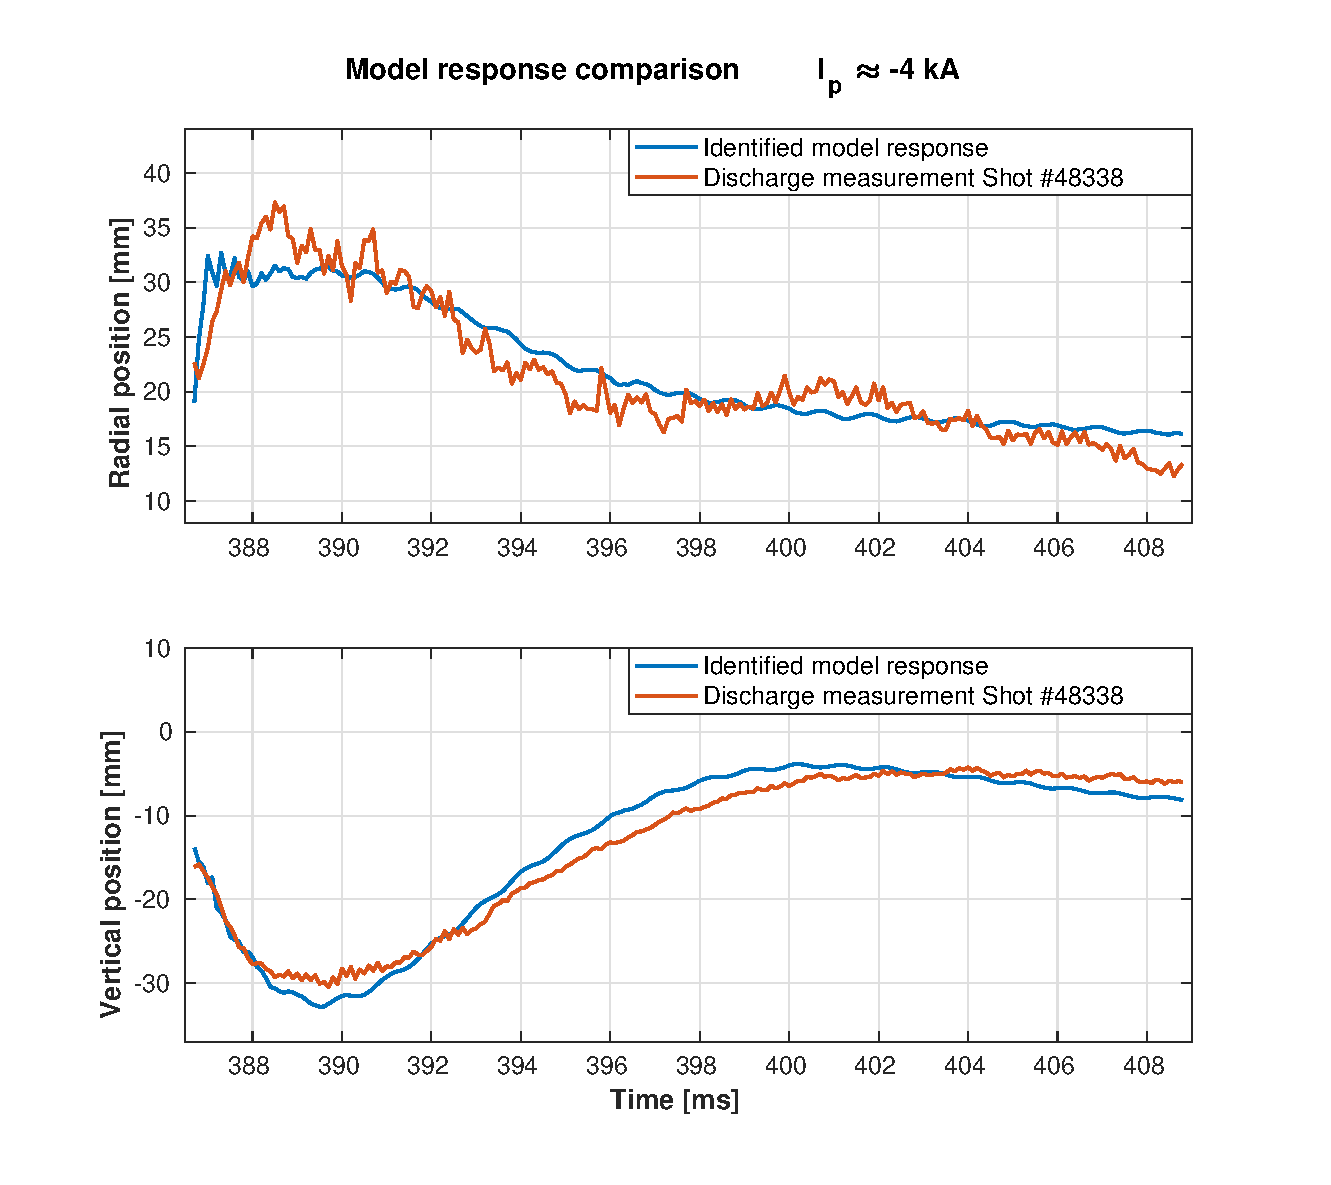
\includegraphics[width=\textwidth]{Chp5/SimResp_338.eps}  
		\caption{\label{cvcv} }
	\end{subfigure}
	~ %add desired spacing between images, e. g. ~, \quad, \qquad, \hfill etc. 
	%(or a blank line to force the subfigure onto a new line)
	\begin{subfigure}[b]{0.55\textwidth}
		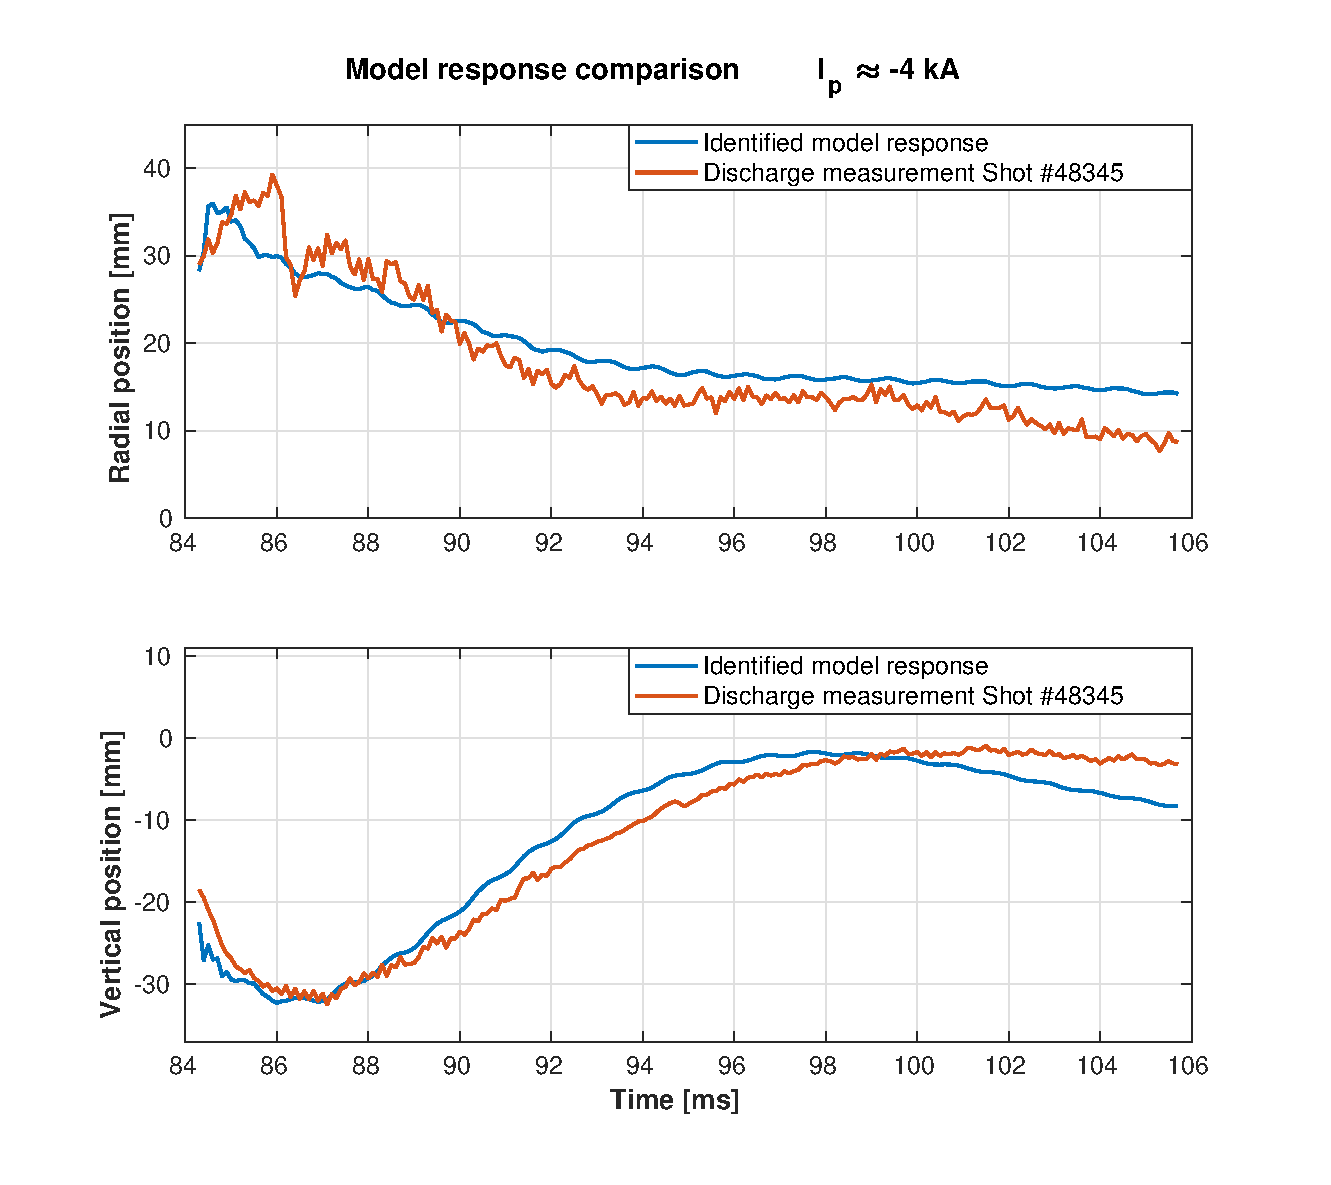
\includegraphics[width=\textwidth]{Chp5/SimResp_345.eps}        
		\caption{\label{vcvc}}
		   \end{subfigure}
	   \caption{Fig. }
\end{figure}


%% Positives
\begin{figure}
	\centering
	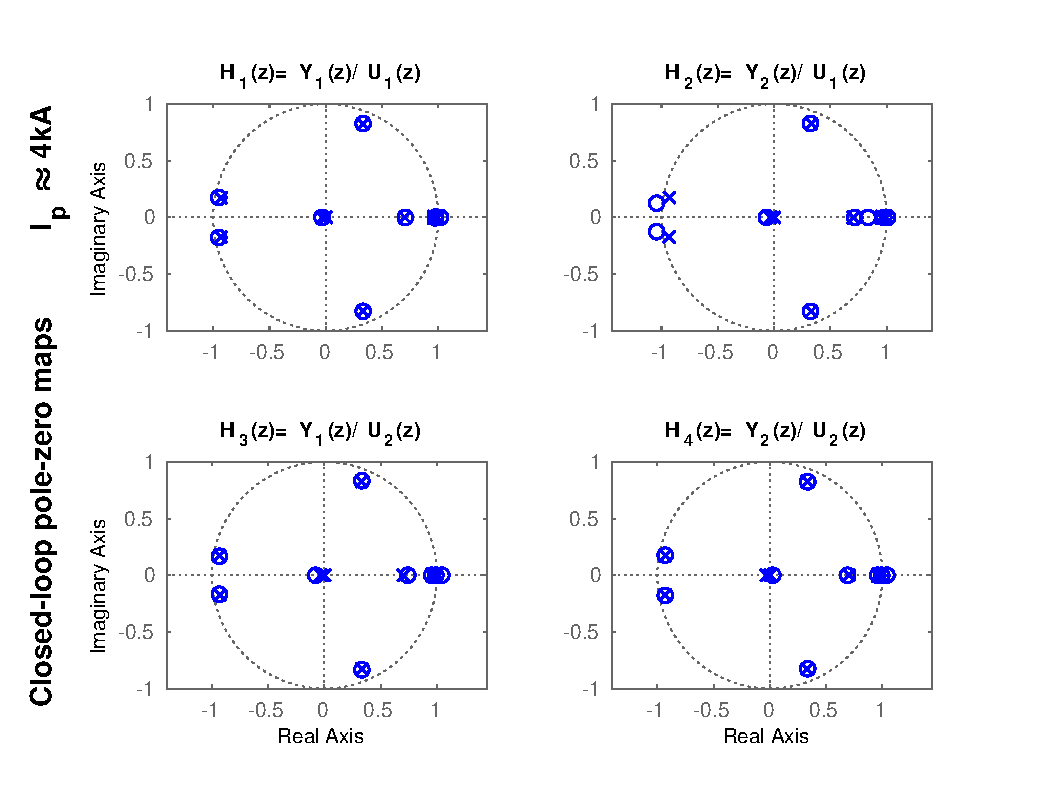
\includegraphics[width=0.85\textwidth]{Chp5/PoleZero/PoleZeroClosePos.eps}
	\label{PoleZeroClosePos}
	\caption{Pole-Zero maps in closed loop for the model when $I_p\approx 4 kA$. Superposition  of poles and zeros can be seen in the four transfer functions.}
\end{figure}	

\begin{figure}
	\centering
	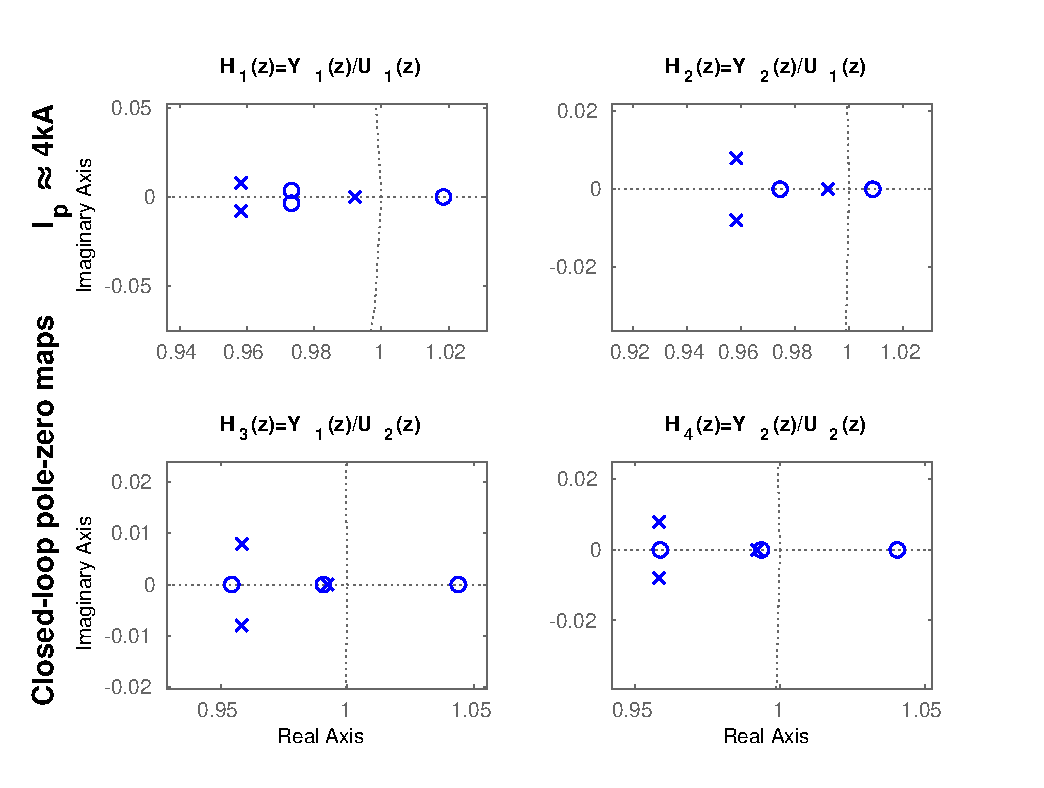
\includegraphics[width=0.85\textwidth]{Chp5/PoleZero/PoleZeroClosePosZoom.eps}
	\label{PoleZeroClosePosZoom}
\end{figure}	


\begin{figure}
	\centering
	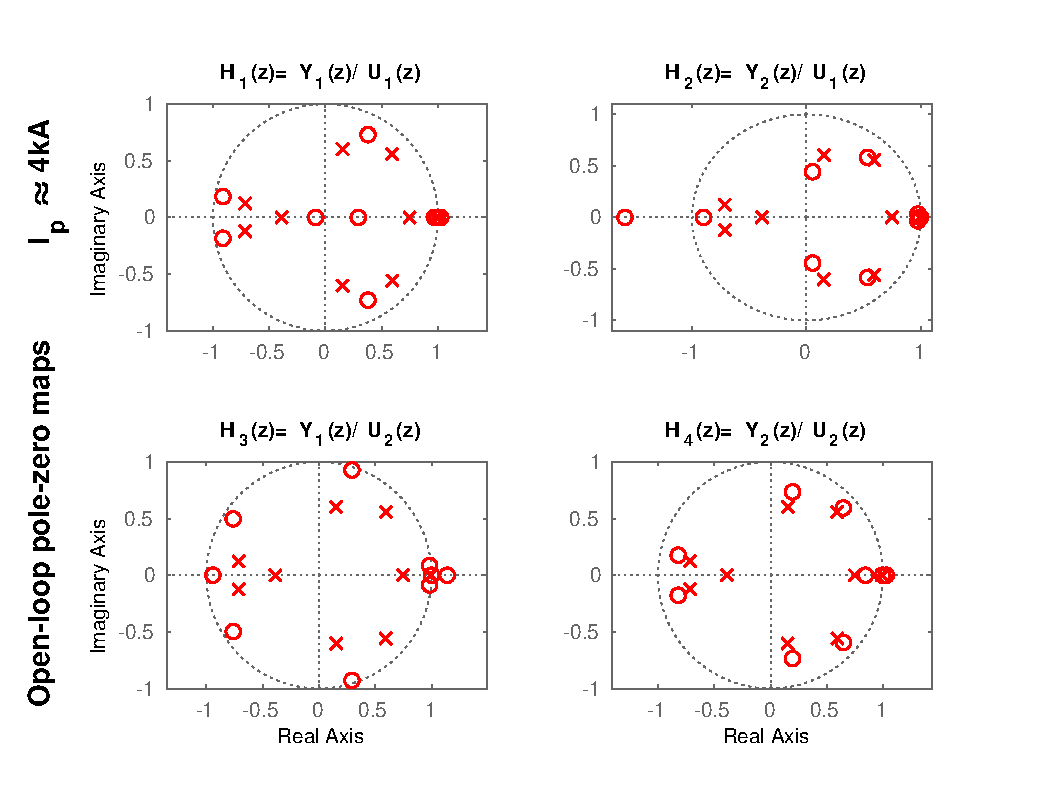
\includegraphics[width=0.85\textwidth]{Chp5/PoleZero/PoleZeroOpenPos.eps}
	\label{PoleZeroOpenPos}
\end{figure}	

\begin{figure}
	\centering
	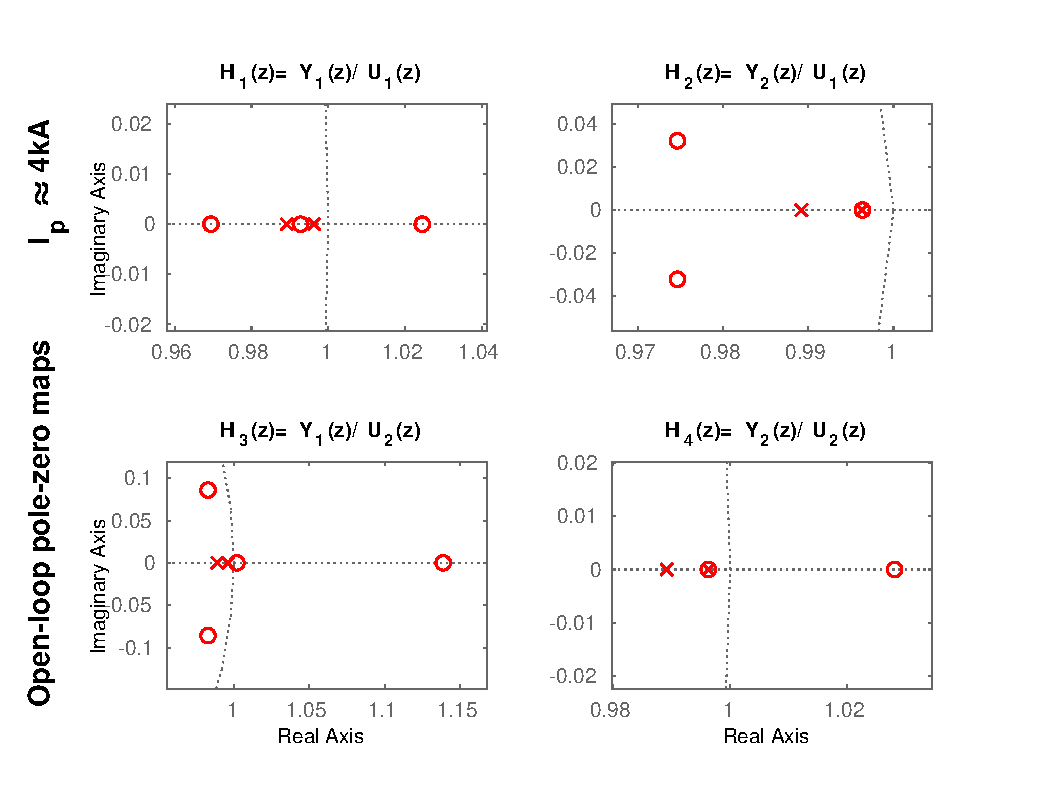
\includegraphics[width=0.85\textwidth]{Chp5/PoleZero/PoleZeroOpenPosZoom.eps}
	\label{PoleZeroOpenPosZoom}
\end{figure}

%% Negatives
\begin{figure}
	\centering
	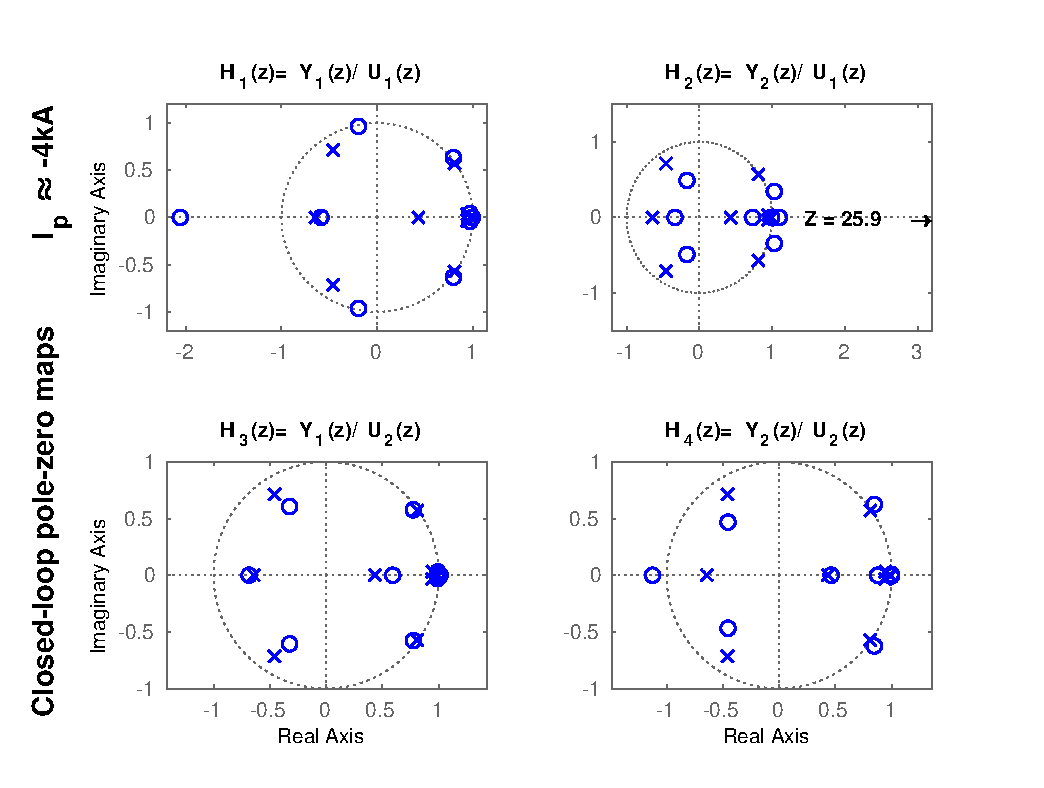
\includegraphics[width=0.85\textwidth]{Chp5/PoleZero/PoleZeroCloseNeg.eps}
	\label{PoleZeroCloseNeg}
\end{figure}	

\begin{figure}
	\centering
	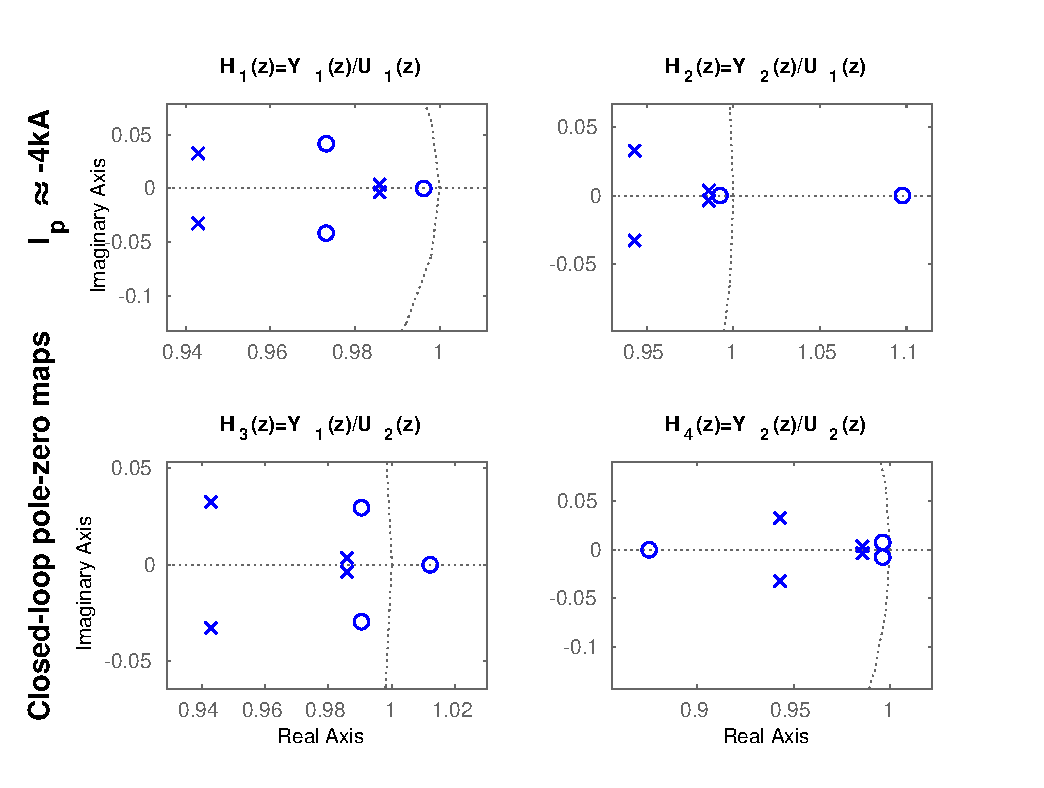
\includegraphics[width=0.85\textwidth]{Chp5/PoleZero/PoleZeroCloseNegZoom.eps}
	\label{PoleZeroCloseNegZoom}
\end{figure}	


\begin{figure}
	\centering
	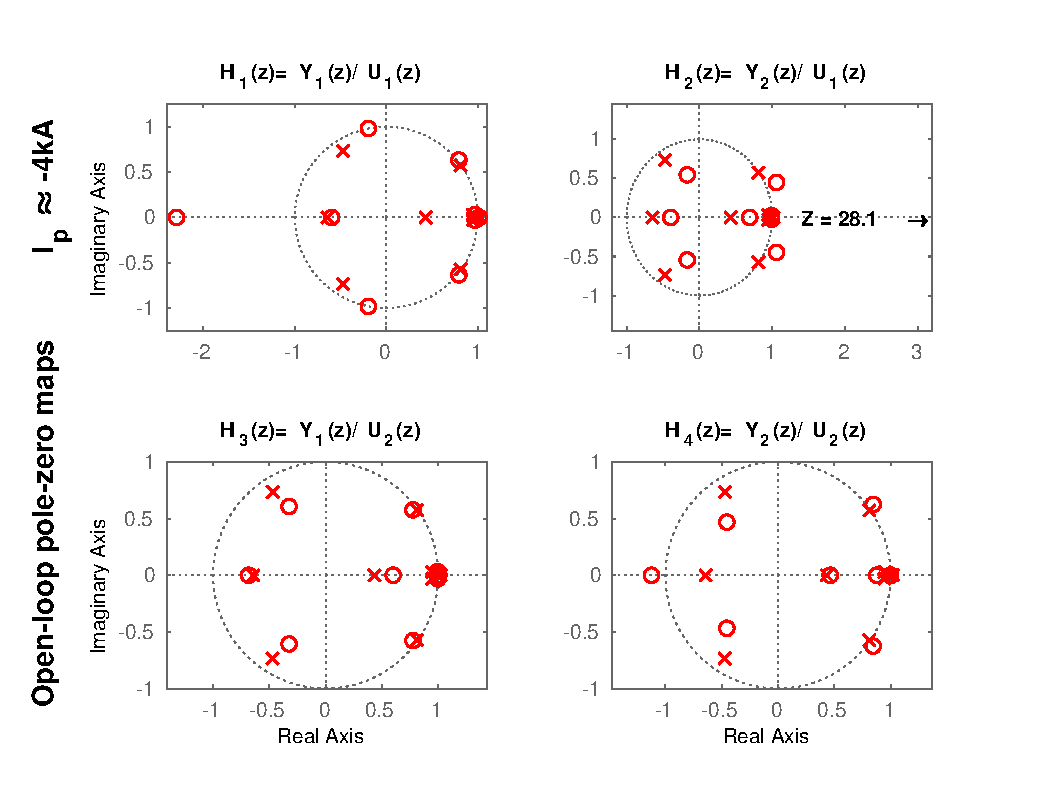
\includegraphics[width=0.85\textwidth]{Chp5/PoleZero/PoleZeroOpenNeg.eps}
	\label{PoleZeroOpenNeg}
\end{figure}	

\begin{figure}
	\centering
	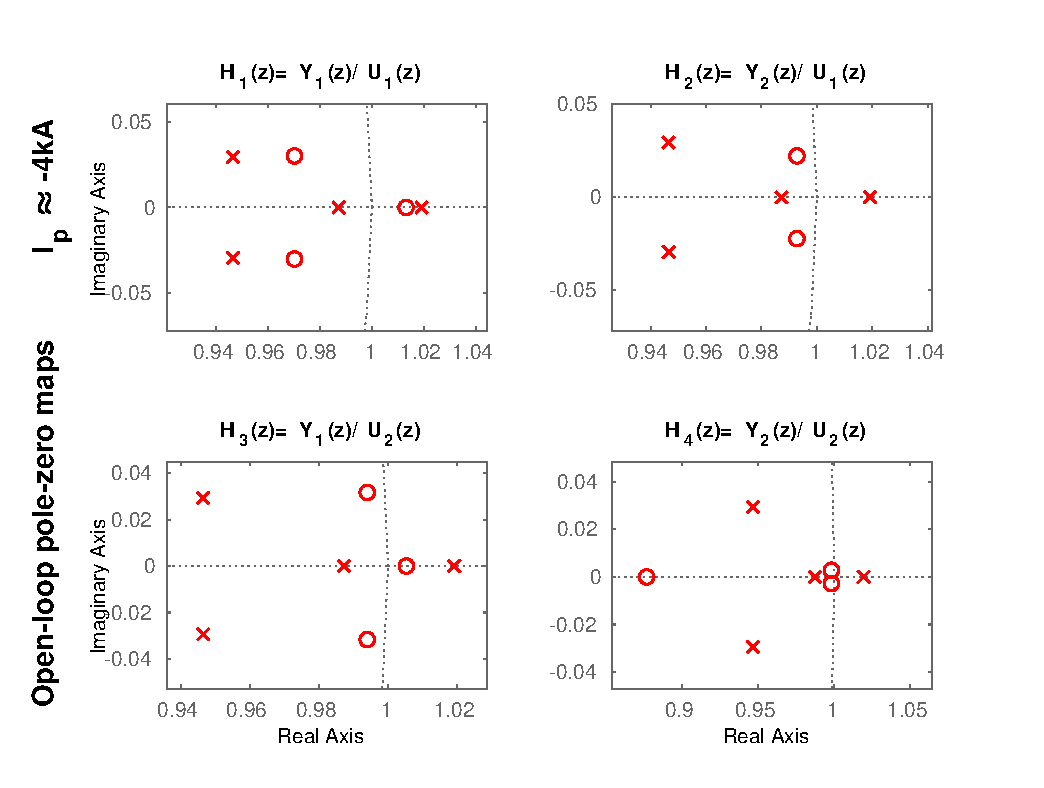
\includegraphics[width=0.85\textwidth]{Chp5/PoleZero/PoleZeroOpenNegZoom.eps}
	\label{PoleZeroOpenNegZoom}
\end{figure}

\subsection{Kalman filter implementation}

\subsection{Multiple-Input Multiple-Output control implementation}
	




\section{Plasma curruent centroid position control results}

This section addresses the latest results from the real-time implementation of control algorithms in ISTTOK. 

\subsection{PID control and LQR control results}

This section addresses obteined the experimental results in ISTTOK's plasma discharges.

\begin{figure}
	\centering
	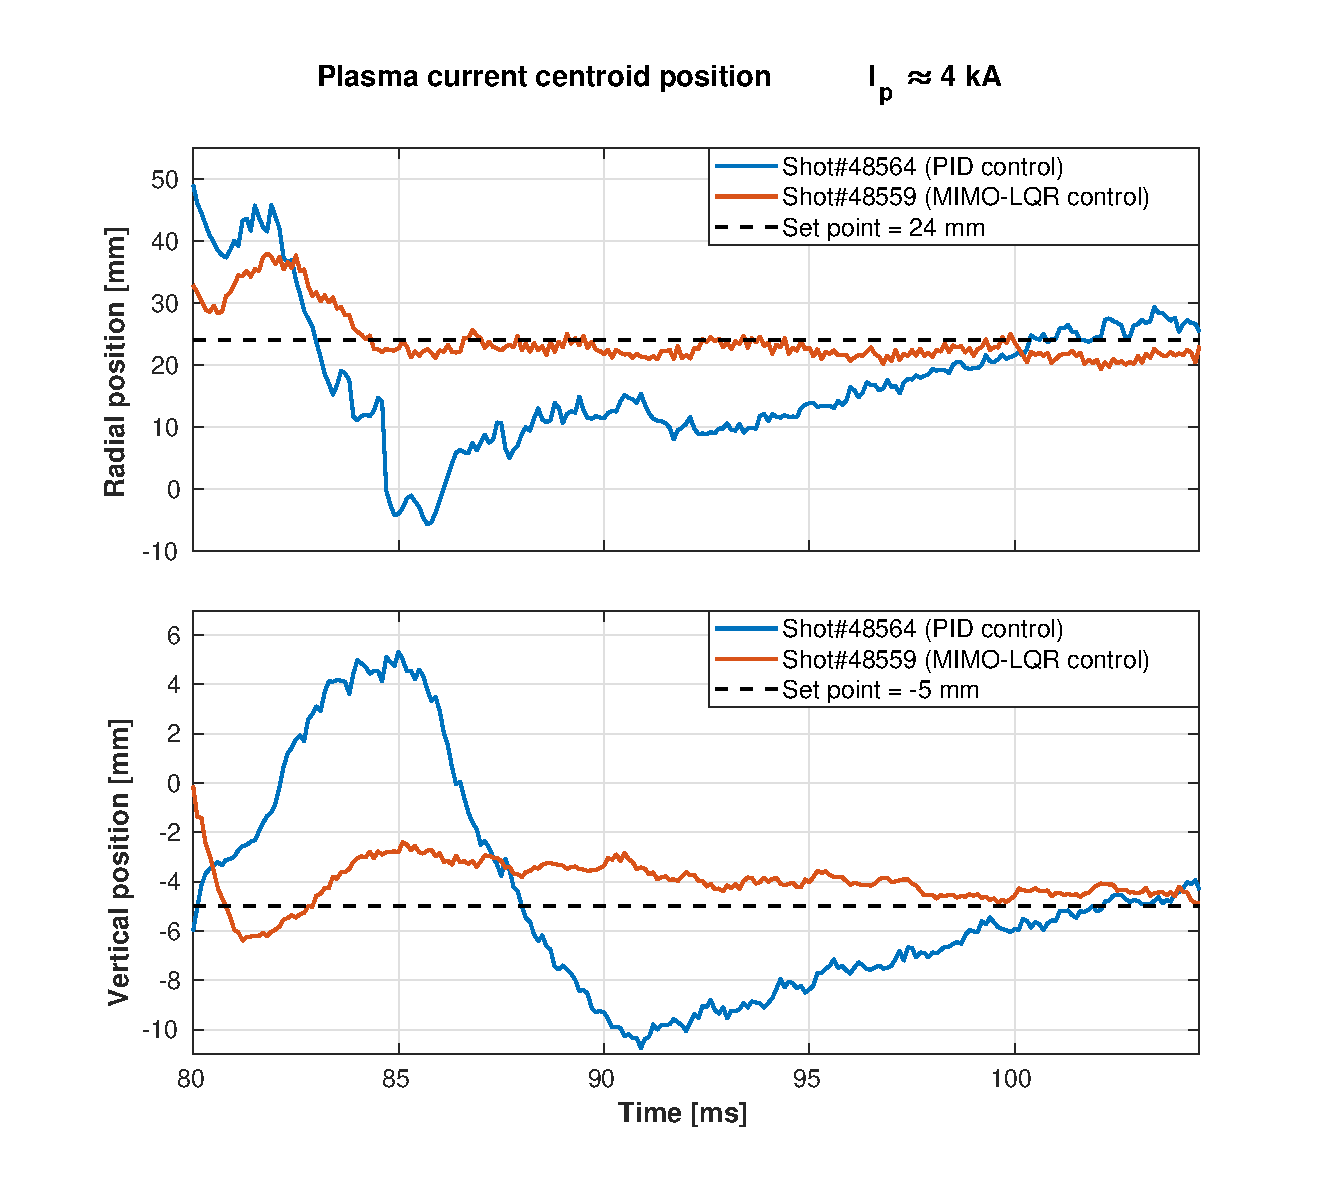
\includegraphics[width=0.8\textwidth]{Chp5/PIDvsMIMO_564_559_2.eps}
	\label{564_559}
\end{figure}

\begin{figure}
	\centering
	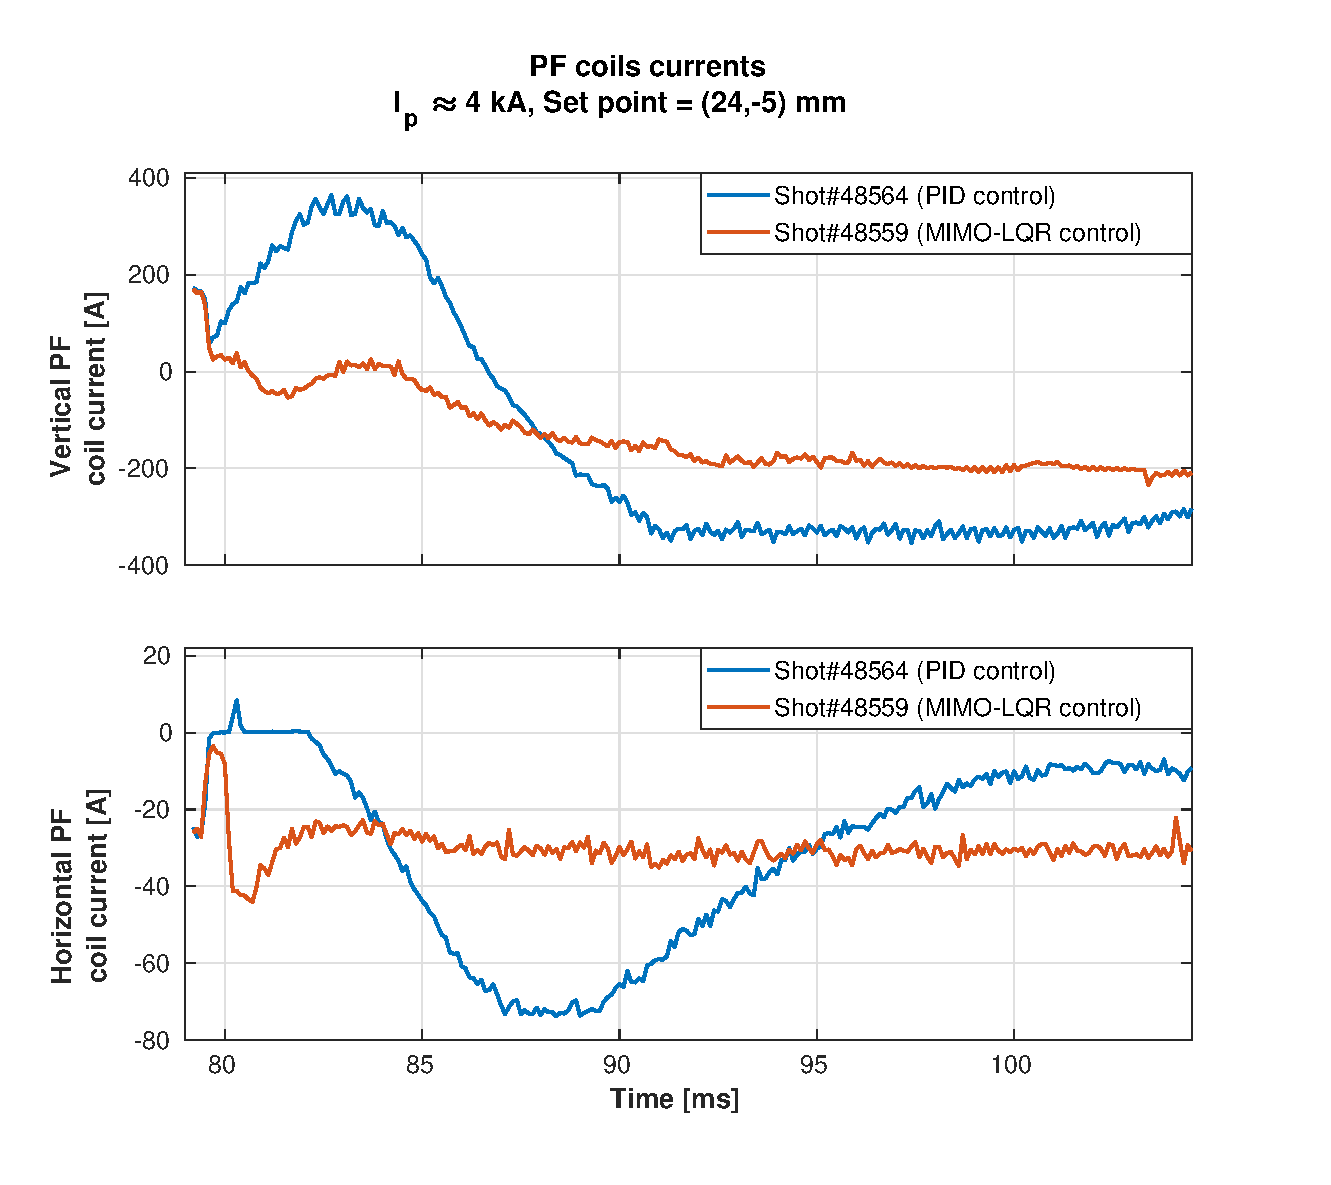
\includegraphics[width=0.8\textwidth]{Chp5/PIDvsMIMO_564_559_curr_2.eps}
	\label{564_559curr}
\end{figure}

\begin{figure}
	\centering
	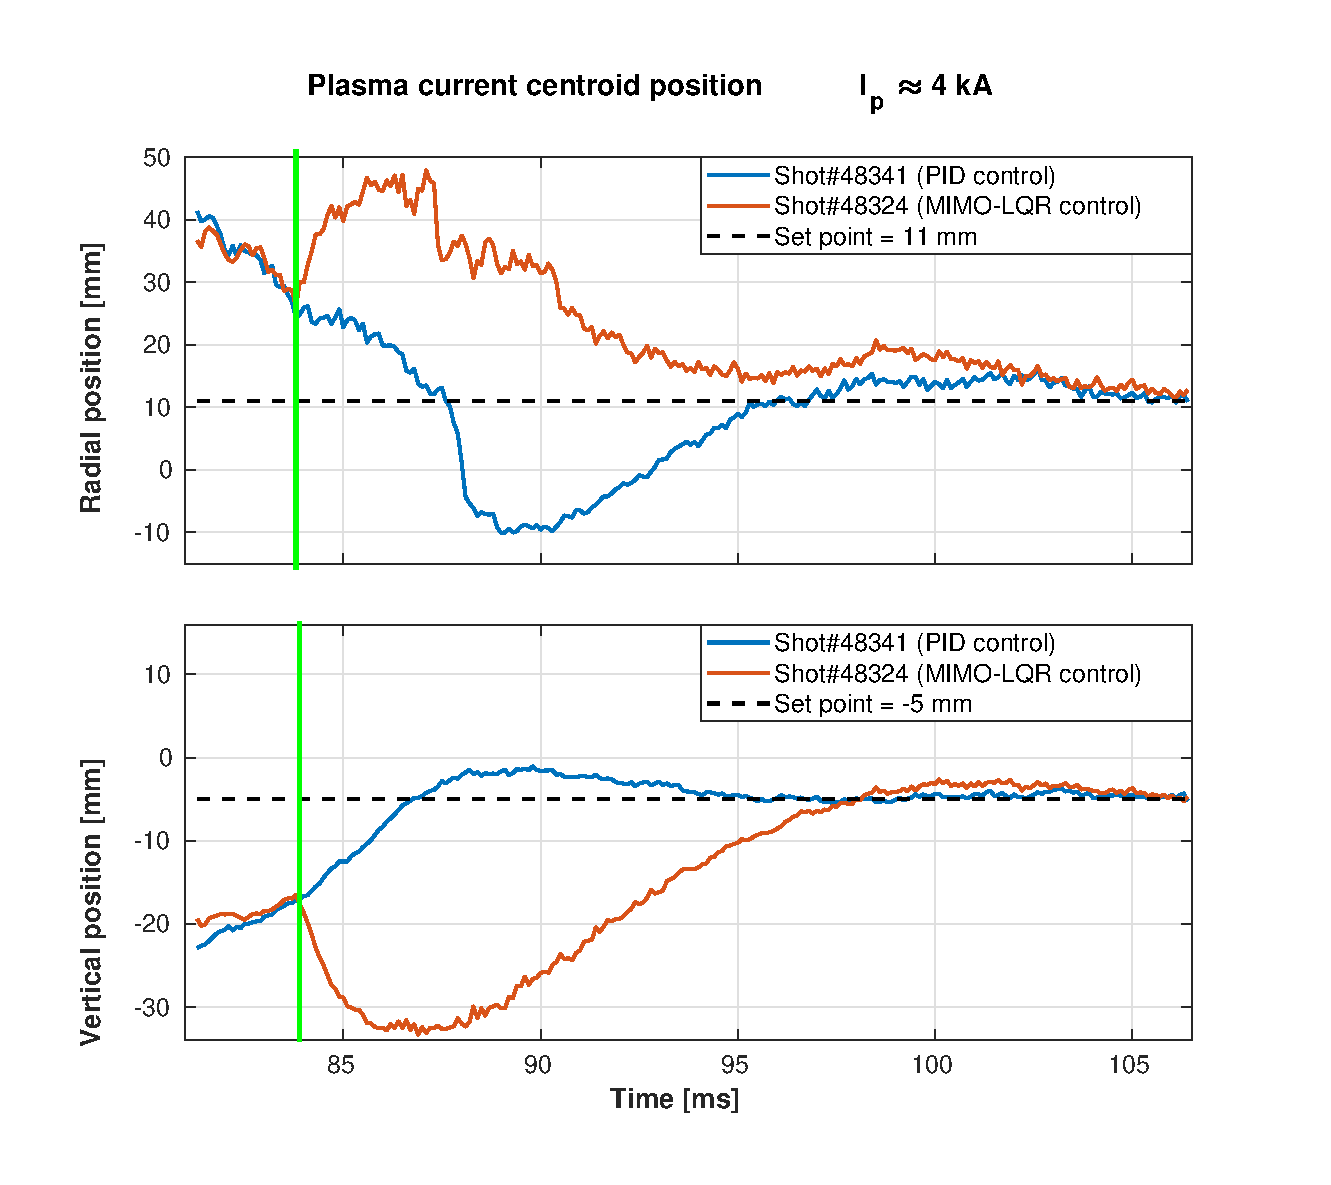
\includegraphics[width=0.8\textwidth]{Chp5/PIDvsMIMO_341_324_2.eps}
	\label{341_342}
\end{figure}

\begin{figure}
	\centering
	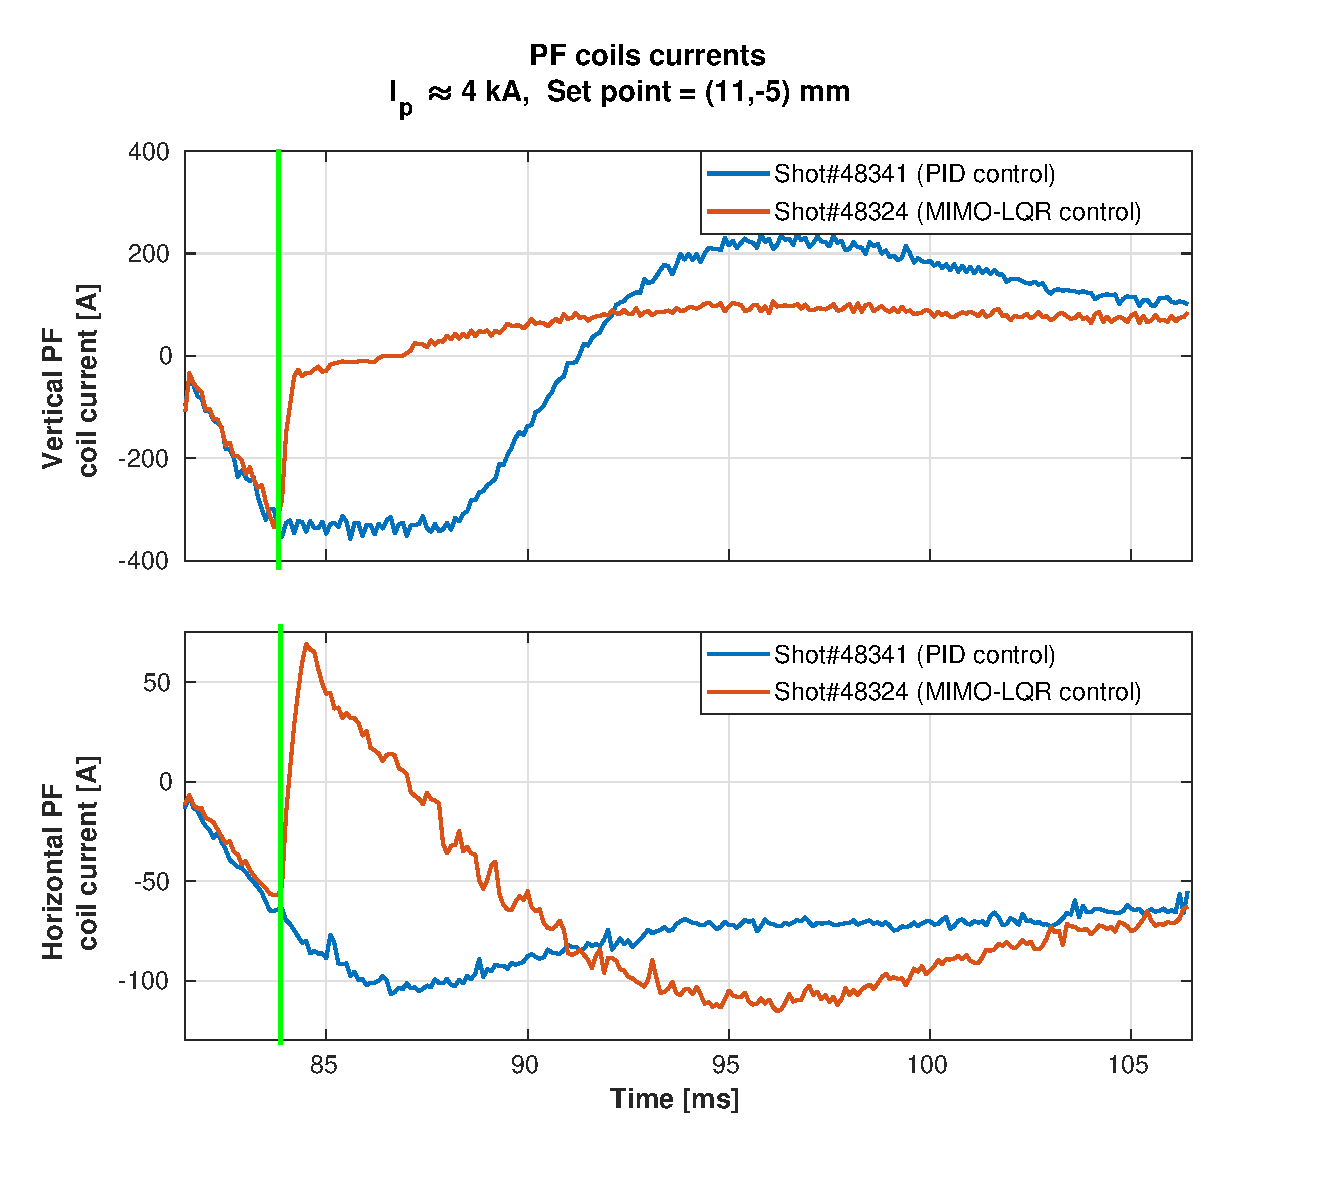
\includegraphics[width=0.8\textwidth]{Chp5/PIDvsMIMO_341_324_curr_2.eps}
	\label{341_342_curr}
\end{figure}


\begin{center}
	\begin{longtable}{||c| c| c| c|c||} 
		\hline
		\textbf{Control} &  \textbf{Shot \#} &\textbf{RMSE (R,z) mm} & \textbf{ Set point (R,z) mm} &\ $\mathbf{I_p}$ \\ [0.5ex] 
		\hline\hline
		PID & 48564 &  (13.73, 4.4102) & (24, -5)&  $\approx 4 kA$ \\ 
		\hline
		MIMO LQR & 48559 & (4.2252, 1.4215 ) & (24, -5)&  $\approx 4 kA$	\\
		\hline
		PID & 48563 & (13.6717,	4.1652)  & (24, -4)& $\approx 4 kA$ \\ 
		\hline
		MIMO LQR & 48561 & (8.1047,	3.2752) & (24, -4)& $\approx 4 kA$ \\
		\hline
		PID & 48556 & (12.0315,	3.3217)  & (32, -5)& $\approx 4 kA$  \\ 
		\hline
		MIMO LQR & 48555 & (4.2618, 2.4698) & (32, -5) &  $\approx 4 kA$ \\
		\hline
		PID & 48551 & (13.9998,	3.3431)  & (27, -5) &  $\approx 4 kA$ \\ 
		\hline
		MIMO LQR & 48554 & (5.9830, 2.0062)  & (27, -5) &  $\approx 4 kA$ \\
		\hline
		PID & 48515 & (6.0178,	2.6123)  & (30, -5) & $\approx 4 kA$ \\ 
		\hline
		MIMO LQR & 48541 & (5.8372,	1.7664) & (30, -5) &  $\approx 4 kA$\\
		\hline
		PID & 48544 & (4.8745,	2.5167)  & (32, -4)& $\approx 4 kA$ \\ 
		\hline
		MIMO LQR & 48542 & (4.4346,	3.6573) & (32, -4)&  $\approx 4 kA$ \\
		\hline
		PID & 48546 & (11.4560, 3.4765)  & (27, -7)&   $\approx 4 kA$\\ 
		\hline
		MIMO LQR & 48548 & (7.6745, 4.1569) & (27, -7)&  $\approx 4 kA$ \\
		\hline
		PID & 48341 & (12.0959,	5.7652)  & (11, -5)& $\approx -4 kA$\\ 
		\hline
		MIMO LQR & 48324 &  (15.4768,	14.3436)& (11, -5)& $\approx -4 kA$ \\
		\hline
		PID & 48340 & ( 11.7701, 5.9599) & (11.2, -5.5)&  $\approx -4 kA$\\ 
		\hline
		MIMO LQR & 48338 & (11.5260,	12.6226) & (11.2, -5.5) &  $\approx -4 kA$\\
		\hline
		PID & 48343 &(15.7675,	5.7453)   & (12, -5)&  $\approx -4 kA$  \\ 
		\hline
		MIMO LQR & 48342 & (14.5168,	14.4329) & (12, -5)&  $\approx -4 kA$  \\
		\hline
		PID & 48346 & (12.4228,	6.1541)  & (12.2, -5.3)& $\approx -4 kA$\\ 
		\hline
		MIMO LQR & 48345 & (9.7513,	13.0338) & (12.2, -5.3)& $\approx -4 kA$ \\
		\hline
		PID & 48349 & (19.3397,	5.5406)  & (11.5, -5.6)&$\approx -4 kA$  \\ 
		\hline
		MIMO LQR & 48348 & (9.1727,	13.1505) & (11.5, -5.6)&$\approx -4 kA$  \\
		\hline
		PID & 48352 &  (15.2181,	6.5395) & (10.8, -4.7) &$\approx -4 kA$ \\ 
		\hline
		MIMO LQR & 48354 & (14.6405,	13.7307) & (10.8, -4.7)& $\approx -4 kA$ \\
		\hline
		PID & 48351 &  (13.4078, 5.8769) & (13.2, -5.6)& $\approx -4 kA$ \\ 
		\hline
		MIMO LQR & 48350 & (13.9320,	14.4940) & (13.2, -5.6)&$\approx -4 kA$  \\[1ex]
		\hline
		\caption{Centroid position RMSE comparison between PID and MIMO-LQR controlled discharges for different set points and plasma current scenarios.}
	\end{longtable}
\label{TableControl}

\end{center}


